\documentclass[10pt,a4paper]{article}
\usepackage[utf8]{inputenc}
\usepackage[italian]{babel}
\usepackage{amsmath}
\usepackage{amsfonts}
\usepackage{amssymb}
\usepackage{graphicx}
\usepackage{siunitx}
\usepackage[left=2cm,right=2cm,top=2cm,bottom=2cm]{geometry}
\newcommand{\rem}[1]{[\emph{#1}]}
\newcommand{\exn}{\phantom{xxx}}
\usepackage[italian]{babel}
\usepackage[utf8]{inputenc}
\usepackage{siunitx}
\usepackage{graphicx}
\usepackage{xcolor}
\usepackage{amsfonts}
\usepackage{amsmath}
\usepackage{amsthm}
\usepackage{tikz}
\usepackage{pgfplots}
\usepackage{enumitem}
\usepackage{siunitx}
\date{\today}
\usetikzlibrary{shapes.geometric,calc,matrix,arrows,snakes,shapes,patterns}
\title{Esercitazione 11B: Flip-Flop e contatori}
\author{Massimo Bilancioni, Alessandro Foligno, Giuseppe Zanichelli}
\begin{document}	
\maketitle
	
\section{ Flip-Flop D-Latch}


\section{ Divisori di frequenza }
Si è montato il circuito in figura come mostrato nell'immagine \textcolor{red}{AGGIUNGERE IMMAGINE}.
Si è verificato il corretto funzionamento del contatore con un impulso a bassa frequenza.

Abbiamo inviato un clock a una frequenza di circa $f\simeq 50 \si{\kilo \hertz}$; nelle immagini che seguono compaiono  rispettivamente $Q0$, $Q1$, $Q2$ e $Q3$ \textcolor{red}{AGGIUNGERE IMMAGINE} (in giallo) sovrapposti al clock (in blu), dalle figure si vede che le frequenze sono effettivamente $1/2$, $1/4$, $1/8$, $1/16$ di $f$.
\begin{figure}[h]
			\centering
			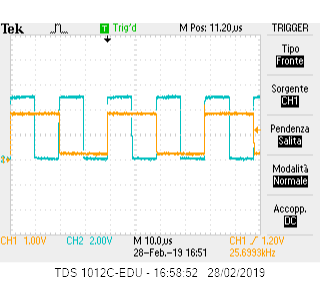
\includegraphics[scale=0.85]{1mezzo}
			\caption{sengale $Q0$ in blu}
			\label{fig:plh}
\end{figure}
\begin{figure}[h]
			\centering
			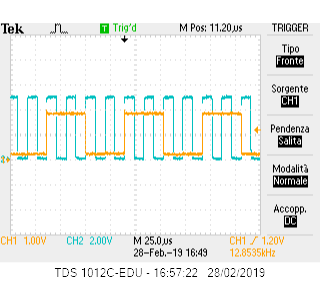
\includegraphics[scale=0.85]{1quarto}
			\caption{sengale $Q1$ in blu}
			\label{fig:plh}
\end{figure}
\begin{figure}[h]
			\centering
			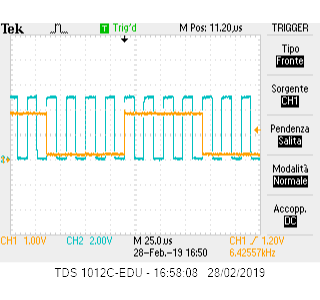
\includegraphics[scale=0.85]{1ottavo}
			\caption{sengale $Q2$ in blu}
			\label{fig:plh}
\end{figure}
Tramite l'oscilloscopio si è poi misurato il ritardo tra la transizione del clock e quella di $Q0$, $Q1$, $Q2$ e $Q3$; in particolare si è misurato l'intervallo temporale che intercorreva da quando la tensione in ingresso passava per il $50\%$ del valore massimo a quando l'uscita passava per  il $50\%$ del valore massimo. Nelle Figure \ref{fig:t1} e \ref{fig:t2} sono mostrati il segnale di clock (in blu) e $Q0$ (in giallo) rispettivamente quando il segnale  $Q0$ passa da alto a basso e da basso ad alto. I ritardi misurati per questa uscita 
sono nel primo caso $t\ped{discesa} = (150 \pm 5)\si{\nano\second}$ e nel secondo  $t\ped{salita} = (30 \pm 5)\si{\nano\second}$.\textcolor{red}{CONTROLLARE COERENZA ERRORI NEI RITARDI PUNTO 2-3}
Per gli altri tre i ritardi sono gli stessi di $Q0$  nei due casi, infatti le quattro uscite sono quasi perfettamente sincrone tra loro; come esempio  mostriamo  i segnali $Q0$ e $Q1$ nella transizione da alto a basso in Figura \ref{fig:q0q1}.
\textcolor{red}{SINCRONIA TRA TRANSIZIONE MISTA?BOH!}
\textcolor{red}{CONFRONTARE TEMPI CON DATASHIIIIIT NON TORNA NULLA!}
\begin{figure}[h]
			\centering
			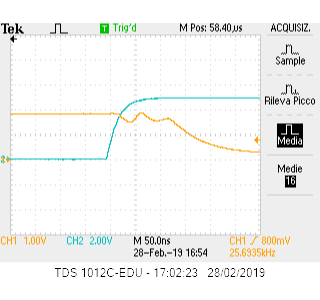
\includegraphics[scale=0.85]{tcounter}
			\caption{ritardo di $Q0$ nel passare da alto a basso}
			\label{fig:t1}
\end{figure}
\begin{figure}[h]
			\centering
			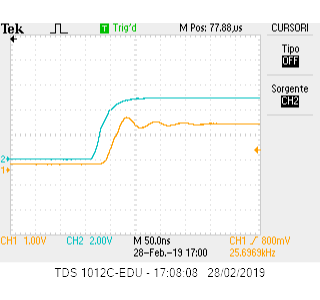
\includegraphics[scale=0.85]{tcounter_1}
			\caption{ritardo di $Q0$ nel passare da basso ad alto}
			\label{fig:t2}
\end{figure}

\begin{figure}[h]
			\centering
			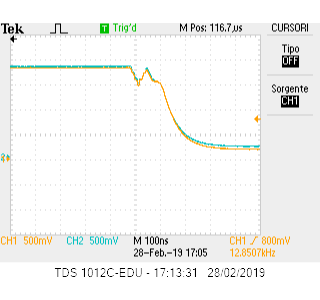
\includegraphics[scale=0.85]{Q0Q1sincroni}
			\caption{quasi perfetta sincronia tra i segnali $Q0$ e $Q1$ quando entrambi diventano bassi}
			\label{fig:q0q1}
\end{figure}
\section{ Shift register con D-Latch}



\end{document}